\printconcepts

\exercise{T/F: Every function has an inverse.}{F}

\exercise{In your own words explain what it means for a function to be ``one to one.''}{Answers will vary.}

\exercise{If $(1,10)$ lies on the graph of $y=f(x)$, what can be said about the graph of $y=f^{-1}(x)$?}{The point $(10,1)$ lies on the graph of $y=f^{-1}(x)$ (assuming $f$ is invertible).}

%\exercise{If $(1,10)$ lies on the graph of $y=f(x)$ and $\fp(1) = 5$, what can be said about $y=f^{-1}(x)$?}{The point $(10,1)$ lies on the graph of $y=f^{-1}(x)$ (assuming $f$ is invertible) and $(f^{-1})'(10) = 1/5$.}

\exercise{If a function doesn't have an inverse, what can we do to help it have an inverse?}{Restrict the domain of the original function so that it is one to one.}

\printproblems

\exerciseset{In Exercises}{, given the graph of $f$, sketch the graph of $f^{-1}$.}{

\exercise{%
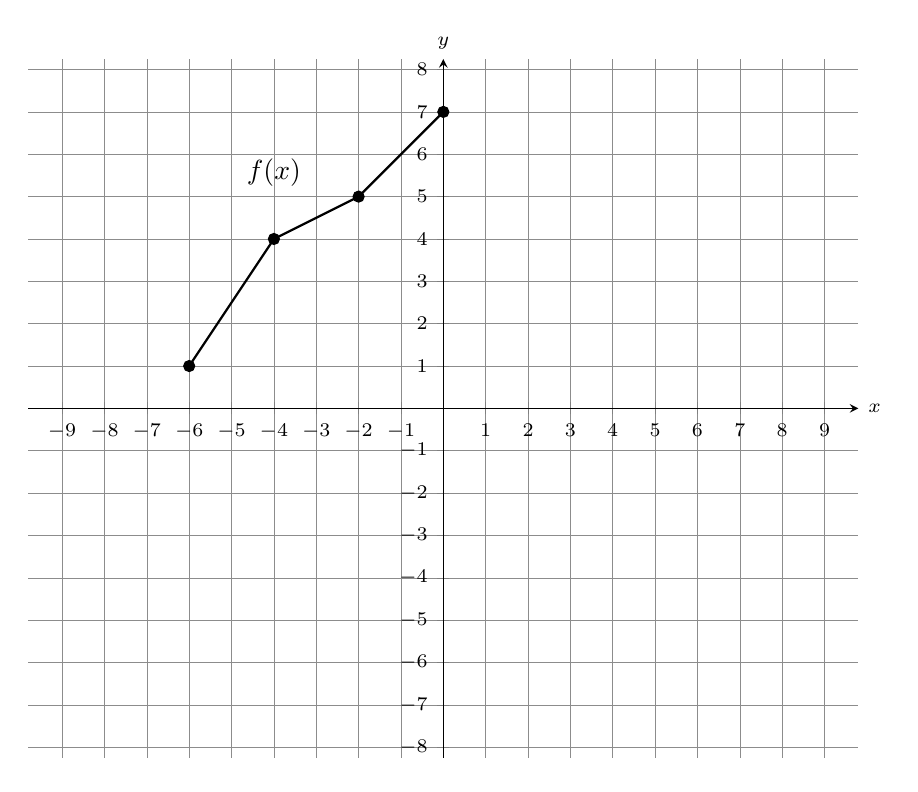
\begin{tikzpicture}
\begin{axis}[width=\linewidth, axis equal,axis x line=middle, axis y line=middle,xmin=-9, xmax=9, ymin=-8.25, ymax=8.25,name=myplot,yticklabel style={{font=\scriptsize}},xticklabel style={{font=\scriptsize}}, xtick={-9,-8,-7,-6,-5,-4,...,5,6,7,8,9}, ytick={-8,-7,-6,-5,-4,...,5,6,7,8},%xticklabel={-8,-7,-6,-5,-4,...,5,6,7,8},
,ymajorgrids=true, xmajorgrids=true, yminorgrids=true, xminorgrids=true,major grid style={line width=.2pt,draw=gray!90}]
\draw[draw={\colorone},thick] (axis cs:-6,1)--(axis cs:-4,4)--(axis cs:-2,5)--(axis cs:0,7);
\addplot[draw={\colorone},mark=*,only marks] coordinates {(-6,1)(-4,4)(-2,5)(0,7)};
\node[above] at (axis cs:-4,5) {$f(x)$};
\end{axis}
\node [right] at (myplot.right of origin) {\scriptsize $x$};
\node [above] at (myplot.above origin) {\scriptsize $y$};
\end{tikzpicture}%
}{%
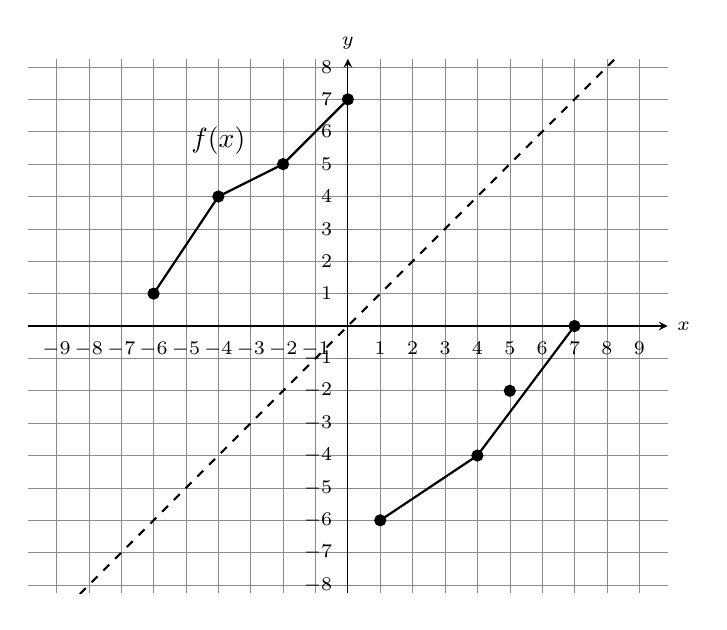
\begin{tikzpicture}
\begin{axis}[width=.8\linewidth, axis equal,axis x line=middle, axis y line=middle,xmin=-9, xmax=9, ymin=-8.25, ymax=8.25,name=myplot,yticklabel style={{font=\scriptsize}},xticklabel style={{font=\scriptsize}}, xtick={-9,-8,-7,-6,-5,-4,...,5,6,7,8,9}, ytick={-8,-7,-6,-5,-4,...,5,6,7,8},%xticklabel={-8,-7,-6,-5,-4,...,5,6,7,8},
,ymajorgrids=true, xmajorgrids=true, yminorgrids=true, xminorgrids=true,major grid style={line width=.2pt,draw=gray!90}]
\draw[draw={\colorone},thick] (axis cs:-6,1)--(axis cs:-4,4)--(axis cs:-2,5)--(axis cs:0,7);
\addplot[draw={\colorone},mark=*,only marks] coordinates {(-6,1)(-4,4)(-2,5)(0,7)};

\draw[draw={\colortwo},thick] (axis cs:1,-6)--(axis cs:4,-4)--(axis cs:7,0);
\addplot[mark=*,only marks,draw={\colortwo}] coordinates {(1,-6)(4,-4)(5,-2)(7,0)};
\addplot[domain=-9:9,black, thick,smooth,dashed] {x};
\node[above] at (axis cs:-4,5) {$f(x)$};
\end{axis}
\node [right] at (myplot.right of origin) {\scriptsize $x$};
\node [above] at (myplot.above origin) {\scriptsize $y$};
\end{tikzpicture}%
}

\exercise{%
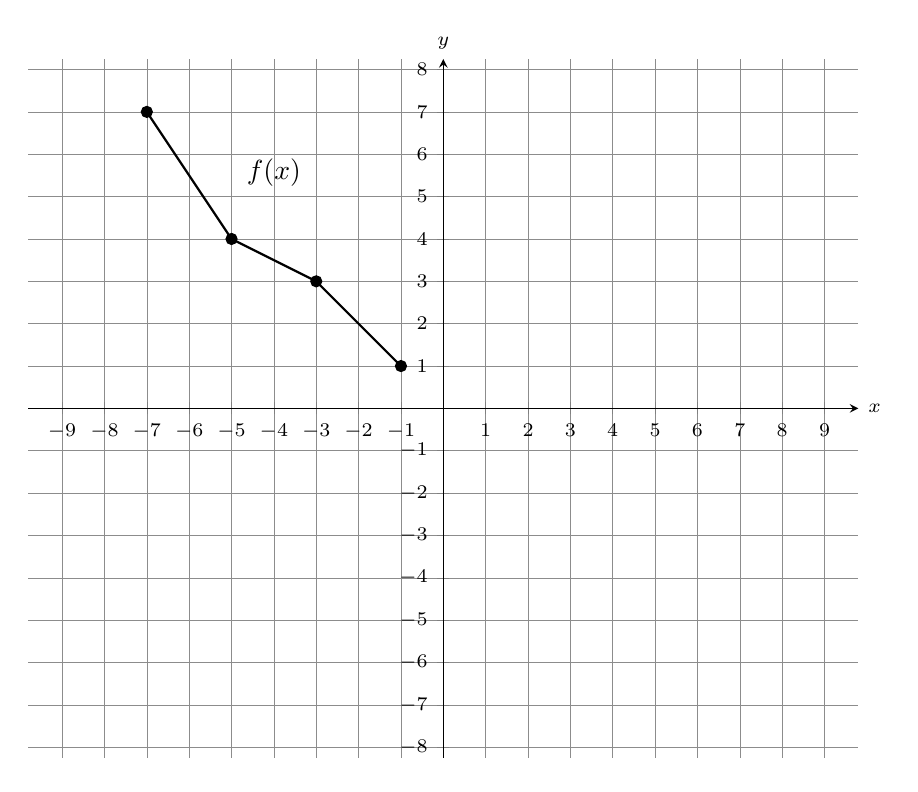
\begin{tikzpicture}
\begin{axis}[width=\linewidth, axis equal,axis x line=middle, axis y line=middle,xmin=-9, xmax=9, ymin=-8.25, ymax=8.25,name=myplot,yticklabel style={{font=\scriptsize}},xticklabel style={{font=\scriptsize}}, xtick={-9,-8,-7,-6,-5,-4,...,5,6,7,8,9}, ytick={-8,-7,-6,-5,-4,...,5,6,7,8},%xticklabel={-8,-7,-6,-5,-4,...,5,6,7,8},
,ymajorgrids=true, xmajorgrids=true, yminorgrids=true, xminorgrids=true,major grid style={line width=.2pt,draw=gray!90}]
\draw[draw={\colorone},thick] (axis cs:-7,7)--(axis cs:-5,4)--(axis cs:-3,3)--(axis cs:-1,1);
\addplot[draw={\colorone},mark=*,only marks] coordinates {(-7,7)(-5,4)(-3,3)(-1,1)};

\node[above] at (axis cs:-4,5) {$f(x)$};
\end{axis}
\node [right] at (myplot.right of origin) {\scriptsize $x$};
\node [above] at (myplot.above origin) {\scriptsize $y$};
\end{tikzpicture}%
}{%
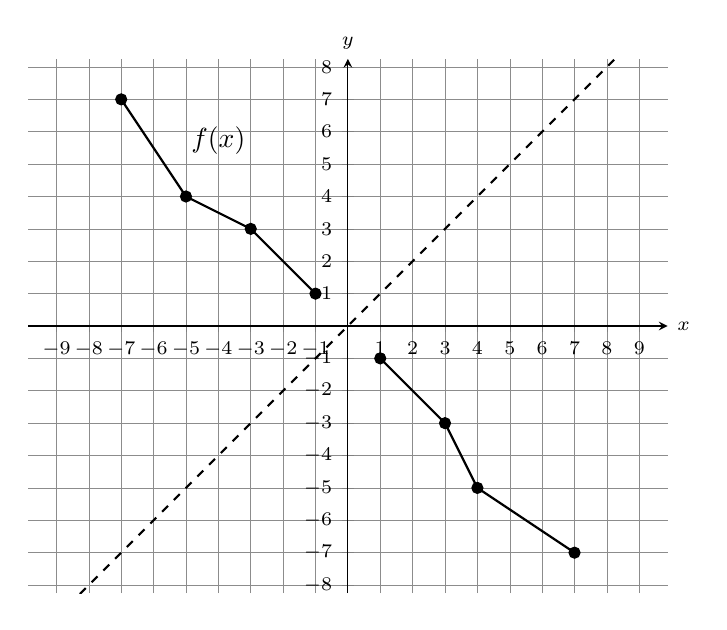
\begin{tikzpicture}
\begin{axis}[width=.8\linewidth, axis equal,axis x line=middle, axis y line=middle,xmin=-9, xmax=9, ymin=-8.25, ymax=8.25,name=myplot,yticklabel style={{font=\scriptsize}},xticklabel style={{font=\scriptsize}}, xtick={-9,-8,-7,-6,-5,-4,...,5,6,7,8,9}, ytick={-8,-7,-6,-5,-4,...,5,6,7,8},%xticklabel={-8,-7,-6,-5,-4,...,5,6,7,8},
,ymajorgrids=true, xmajorgrids=true, yminorgrids=true, xminorgrids=true,major grid style={line width=.2pt,draw=gray!90}]
\draw[draw={\colortwo},thick] (axis cs:-7,7)--(axis cs:-5,4)--(axis cs:-3,3)--(axis cs:-1,1);
\addplot[mark=*,only marks] coordinates {(-7,7)(-5,4)(-3,3)(-1,1)};

\addplot[domain=-9:9,black, thick,smooth,dashed] {x};
\draw[draw={\colortwo},thick] (axis cs:7,-7)--(axis cs:4,-5)--(axis cs:3,-3)--(axis cs:1,-1);
\addplot[draw={\colorone},mark=*,only marks] coordinates {(7,-7)(4,-5)(3,-3)(1,-1)};
\node[above] at (axis cs:-4,5) {$f(x)$};
\end{axis}
\node [right] at (myplot.right of origin) {\scriptsize $x$};
\node [above] at (myplot.above origin) {\scriptsize $y$};
\end{tikzpicture}%
}

}

\begin{exerciseset}{In Exercises}{, verify that the given functions are inverses.}

\exercise{$f(x) = 2x+6$ and $g(x) = \frac12x-3$}{Compose $f(g(x))$ and $g(f(x))$ to confirm that each equals $x$.}

\exercise{$f(x) = x^2+6x+11$, $x\geq-3$ and $g(x) = \sqrt{x-2}-3$, $x\geq 2$}{Compose $f(g(x))$ and $g(f(x))$ to confirm that each equals $x$.}

% cut for parity
%\exercise{$f(x)=x^2+6x+11$, $x\le 3$ and $g(x)=-\sqrt{x-2}-3$, $x\ge 2$.}{Compose $f(g(x))$ and $g(f(x))$ to confirm that each equals $x$.}

\exercise{$\ds f(x) = \frac{3}{x-5}$, $x\neq 5$ and  $\ds g(x) = \frac{3+5x}{x}$, $x\neq 0$}{Compose $f(g(x))$ and $g(f(x))$ to confirm that each equals $x$.}

\exercise{$\ds f(x) = \frac{x+1}{x-1}$, $x\neq 1$ and $g(x) = f(x)$}{Compose $f(g(x))$ and $g(f(x))$ to confirm that each equals $x$.}

\end{exerciseset}


\exerciseset{In Exercises}{, find the inverse of the given function. Indicate how the domain can be restricted if necessary.}{

\exercise{$f(x)=7x-2$}{$f^{-1}(x)=(x+2)/7$}

\exercise{$g(x)=\sqrt{9-x^2}$}{$g^{-1}(x)=\pm\sqrt{9-x^2}$ on $[0,3]$.  If the domain of $g$ is restricted to $[0,3]$, then we use $+$.  If the domain is restricted to $[-3,0]$, then we use $-$.}

\exercise{$r(t)=t^2-6t+9$}{$r^{-1}(t)=3\pm\sqrt t$.  If the domain of $r$ is restricted to $[3,\infty)$, then we use $+$.  If the domain is restricted to $(-\infty,3]$, then we use $-$.}

}

\exerciseset{In Exercises}{, simplify the expression.}{

\exercise{$\sin\Bigl(\tan^{-1}\frac{x}{\sqrt{4-x^2}}\Bigr)$}{$x/2$}

\exercise{$\tan\Bigl(\sin^{-1}\frac{x}{\sqrt{x^2+4}}\Bigr)$}{$x/2$}

\exercise{$\cos\Bigl(\sin^{-1}\frac{5}{\sqrt{x^2+25}}\Bigr)$}{$x/\sqrt{x^2+25}$}

\exercise{$\cot\Bigl(\cos^{-1}\frac{3}{\sqrt{x}}\Bigr)$}{$3/\sqrt{x-3}$}

}

\exercise{Show that for any $x$ in the domain of $\sec^{-1}$ we have $\sec^{-1}x=\cos^{-1}\frac1x$.}{}

\exercise{Show that for $\abs x\le1$ we have $\cos^{-1}x=\frac\pi2-\sin^{-1}x$.\\
Hint: Recall the cofunction identity $\cos\theta=\sin(\frac\pi2-\theta)$ for all $\theta$.}{}

\exercise{Show that for any $x$ we have $\cot^{-1}x=\frac\pi2-\tan^{-1}x$.}{}

\exercise{Show that for $\abs x\ge1$ we have $\csc^{-1}x=\frac\pi2-\sec^{-1}x$.}{}

\exercise{A mass attached to a spring oscillates vertically about the equilibrium position $y=0$ according to the function $y(t)=e^{-t}(\cos(\sqrt3t)+\frac1{\sqrt3}\sin(\sqrt3t))$. Find the first positive time $t$ for which $y(t)=0$.}{$2\pi/3\sqrt3$}


%\input{exercises/02_07_exset_02}
%\exerciseset{In Exercises}{, compute the derivative of the given function.}{

\exercise{$h(t) = \sin^{-1} (2t)$}{$h'(t) = \frac{2}{\sqrt{1-4t^2}}$}

\exercise{$f(t) = \sec^{-1} (2t)$}{$\fp(t) = \frac{1}{\abs t\sqrt{4t^2+1}}$}

\exercise{$g(x)=\tan^{-1} (2x)$}{$g'(x) = \frac{2}{1+4x^2}$}

\exercise{$f(x) =x\sin^{-1}x$}{$\fp(x) = \frac{x}{\sqrt{1-x^2}}+\sin ^{-1}(x)$}

\exercise{$g(t) = \sin t\cos^{-1}t$}{$g'(t) = \cos ^{-1}(t) \cos (t)-\frac{\sin (t)}{\sqrt{1-t^2}}$}

\exercise{$\ds h(x) = \frac{\sin^{-1}x}{\cos^{-1}x}$}{$h'(x)=\frac{\sin ^{-1}(x)+\cos ^{-1}(x)}{\sqrt{1-x^2} \cos ^{-1}(x)^2}$}

\exercise{$g(x) = \tan^{-1}(\sqrt{x})$}{$g'(x) = \frac{1}{\sqrt{x} (2 x+2)}$}

\exercise{$f(x) =\sec^{-1}(1/x)$}{$\fp(x) = -\frac{1}{\sqrt{1-x^2}}$}

\exercise{$f(x) =\sin (\sin^{-1}x)$}{\begin{enumerate}
\item		$f(x) = x$, so $\fp(x) = 1$
\item		$\fp(x) = \cos(\sin^{-1}x)\frac{1}{\sqrt{1-x^2}} = 1$.
\end{enumerate}}

}

%\input{exercises/02_07_exset_04}
%\input{exercises/02_07_exset_05}
%%\begin{exerciseset}{In Exercises}{, find the requested derivative.}

\exercise{$f(x) = x\sin x$; find $\fpp(x)$.}{$\fpp(x) = 2\cos x - x\sin x$}

\exercise{$f(x) = x\sin x$; find $f\,^{(4)}(x)$.}{$f^{(4)}(x) = -4\cos x+ x\sin x$}

\exercise{$f(x) = \csc x$; find $\fpp(x)$.}{$\fpp(x) = \cot^2x\csc x + \csc^3 x$}

\exercise{$f(x) = (x^3-5x+2)(x^2+x-7)$; find $f\,^{(8)}(x)$.}{$f^{(8)} = 0$}

\end{exerciseset}

%%\exerciseset{In Exercises}{, use the graph of $f(x)$ to sketch $\fp(x)$.}{

\exercise{\begin{minipage}[]{\linewidth}
\myincludegraphics[scale=.8]{figures/fig02_04_ex_43}
\end{minipage}
}{\mbox{}\\[-\baselineskip]\myincludegraphics[scale=.8]{figures/fig02_04_ex_43a}
}

\exercise{\begin{minipage}[]{\linewidth}
\myincludegraphics[scale=.8]{figures/fig02_04_ex_44}
\end{minipage}
}{\mbox{}\\[-\baselineskip]\myincludegraphics[scale=.8]{figures/fig02_04_ex_44a}
}

\exercise{\begin{minipage}[]{\linewidth}
\myincludegraphics[scale=.8]{figures/fig02_04_ex_45}
\end{minipage}
}{\mbox{}\\[-\baselineskip]\myincludegraphics[scale=.8]{figures/fig02_04_ex_45a}
}

}

%\printreview
%\exercise{Find $\dfrac{dy}{dx}$, where $x^2y-y^2x = 1$. }{ $\frac{dy}{dx} = \frac{y (y-2 x)}{x (x-2 y)}$}

%\exercise{Find the equation of the line tangent to the graph of $x^2+y^2+xy=7$ at the point $(1,2)$. }{ $y=-\frac45(x-1)+2$}

%\exercise{Let $f(x) = x^3+x$. Evaluate $\ds \lim_{s\to 0} \frac{f(x+s)-f(x)}{s}$.}{ $3x^2+1$}

%%\exercise{Approximate the value of $(3.01)^4$ using the tangent line to $f(x) = x^4$ at $x=3$.}{The tangent line to $f(x) = x^4$ at $x=3$ is $y=108(x-3)+81$; thus $(3.01)^4 \approx y(3.01) = 108(.01)+81 = 82.08$. }
